\pdfoutput=1
\documentclass[a4paper,pdflatex,ja=standard]{bxjsarticle}

% ---Setting about the geometry of the document----
% \usepackage{a4wide}
% \pagestyle{empty}

% ---Physics and Math Packages---
\usepackage{amssymb,amsfonts,amsthm,mathtools}
\usepackage{physics,braket,bm}

% ---underline---
\usepackage{ulem}

% --- sorround the texts or equations
% \usepackage{fancybox,ascmac}

% ---settings of theorem environment---
% \usepackage{amsthm}
% \theoremstyle{definition}

% ---settings of proof environment---
% \renewcommand{\proofname}{\textbf{証明}}
% \renewcommand{\qedsymbol}{$\blacksquare$}

% ---Ignore the Warnings---
\usepackage{silence}
\WarningFilter{latexfont}{Some font shapes,Font shape}

% ---Insert the figure (If insert the `draft' at the option, the process becomes faster)---
% \usepackage{graphicx}
% \usepackage{subcaption}

% ----Add a link to a text---
\usepackage{url}
\usepackage{xcolor,hyperref}
\hypersetup{colorlinks=true,citecolor=orange,linkcolor=blue,urlcolor=magenta}
\usepackage{bxcjkjatype}

% ---Tikz---
\usepackage{tikz,pgf,pgfplots,circuitikz}
\pgfplotsset{compat=1.15}
\usetikzlibrary{intersections,arrows.meta,angles,calc,3d,decorations.pathmorphing}

% ---Add the section number to the equation, figure, and table number---
\makeatletter
   \renewcommand{\theequation}{\thesection.\arabic{equation}}
   \@addtoreset{equation}{section}
   
   \renewcommand{\thefigure}{\thesection.\arabic{figure}}
   \@addtoreset{figure}{section}
   
   \renewcommand{\thetable}{\thesection.\arabic{table}}
   \@addtoreset{table}{section}
\makeatother

% ---enumerate---
\renewcommand{\labelenumi}{$(\arabic{enumi})$}
% \renewcommand{\labelenumii}{$(\arabic{enumii})$}

% ---Index---
%\usepackage{makeidx}
%\makeindex 

% ---Fonts---
\renewcommand{\familydefault}{\sfdefault}

% ---Title---
\title{早稲田大学\ 2018年\ 物理学専攻\ 院試\ 解答例}
\author{ミヤネ}
\date{最終更新:\today}

\newcommand{\prb}[2]{
  \clearpage
  \phantomsection
  \addcontentsline{toc}{section}{問題 #1: #2}
  \section*{問題番号\fbox{#1}\ (#2)}
  \setcounter{section}{#1}
  \setcounter{equation}{0}
}

\begin{document}

\maketitle

\tableofcontents
\clearpage

\prb{3}{力学}

\begin{enumerate}
  \item 
  $x$軸方向の運動方程式は
  \begin{equation}
    m\dv[2]{x}{t}
    =
    -mg\sin\theta
  \end{equation}
  なので,$\sin\theta\sim\theta\sim x/l$より,$x(0)=a,\dot{x}(0)=0$で解けば
  \begin{equation}
    x(t)
    =
    a\cos\left( \sqrt{\frac{g}{l}t} \right)
    .
  \end{equation}

  \item 
  速度は
  \begin{equation}
    \dot{x}(t)
    =
    -a\sqrt{\frac{g}{l}}\sin\left( \sqrt{\frac{g}{l}t} \right)
  \end{equation}
  なので,
  \begin{equation}
    K(t)
    =
    \frac{ma^2g}{2l}\sin^2\left( \sqrt{\frac{g}{l}t} \right)
    .
  \end{equation}
  よって,最大値は
  \begin{equation}
    K_{\max}
    =
    \frac{ma^2g}{2l}
  \end{equation}
  であり,平均は
  \begin{equation}
    \bar{K}
    =
    \frac{2\pi}{\omega}
    \int_{0}^{2\pi/\omega}\dd t^{\prime}\ 
    K(t)
    =
    \frac{1}{2}\cdot\frac{ma^2g}{2l}
    =
    \frac{1}{2}K_{\max}
    .
  \end{equation}

  \item 
  変換則は
  \begin{equation}
    \begin{pmatrix}
      x \\
      y
    \end{pmatrix}
    =
    \begin{pmatrix}
      \cos\omega t & -\sin\omega t \\
      \sin \omega t & \cos \omega t
    \end{pmatrix}
    \begin{pmatrix}
      x' \\
      y'
    \end{pmatrix}
  \end{equation}
  なので,
  \begin{equation}
    \begin{pmatrix}
      \ddot{x} \\
      \ddot{y}
    \end{pmatrix}
    =
    \begin{pmatrix}
      \cos\omega t & -\sin\omega t \\
      \sin \omega t & \cos \omega t
    \end{pmatrix}
    \begin{pmatrix}
      \ddot{x}^{\prime} \\
      \ddot{y}^{\prime}
    \end{pmatrix}
    -
    2\omega
    \begin{pmatrix}
      \sin\omega t & \cos\omega t \\
      -\cos \omega t & \sin \omega t
    \end{pmatrix}
    \begin{pmatrix}
      \dot{x}^{\prime} \\
      \dot{y}^{\prime}
    \end{pmatrix}
    -
    \omega^2
    \begin{pmatrix}
      \cos\omega t & -\sin\omega t \\
      \sin \omega t & \cos \omega t
    \end{pmatrix}
    \begin{pmatrix}
      x^{\prime} \\
      y^{\prime}
    \end{pmatrix}
  \end{equation}
  である.これを$\ddot{x}^{\prime},\ddot{y}^{\prime}$について解けば
  \begin{align}
    \begin{pmatrix}
      \ddot{x}^{\prime} \\
      \ddot{y}^{\prime}
    \end{pmatrix}
    &=
    \begin{pmatrix}
      \cos\omega t & \sin\omega t \\
      -\sin\omega t & \cos\omega t
    \end{pmatrix}
    \begin{pmatrix}
      \ddot{x} \\
      \ddot{y}
    \end{pmatrix}
    +
    2\omega
    \begin{pmatrix}
      \dot{y}^{\prime} \\
      -\dot{x}^{\prime}
    \end{pmatrix}
    +
    \omega^2
    \begin{pmatrix}
      x^{\prime} \\
      y^{\prime}
    \end{pmatrix}
    \nonumber
    \\
    &=
    \frac{1}{m}
    \bm{F}^{\prime}
    +
    2\omega
    \begin{pmatrix}
      \dot{y}^{\prime} \\
      -\dot{x}^{\prime}
    \end{pmatrix}
    +
    \omega^2
    \begin{pmatrix}
      x^{\prime} \\
      y^{\prime}
    \end{pmatrix}
    \label{EOM}
  \end{align}
  である.

  \item 
  (\ref{EOM})のうち,第1項が物体が受ける力.第2項は速度に依存しているのでコリオリ力.第3項は位置に依存しているので遠心力である.

  \item 
  おもりに働く力は,$\text{O}^{\prime}-x^{\prime}y^{\prime}z^{\prime}$系では
  \begin{equation}
    \bm{F}^{\prime}
    =
    -\frac{g}{l}r(t)
    \begin{pmatrix}
      x^{\prime} \\
      y^{\prime}
    \end{pmatrix}
  \end{equation}
  と書けるので,運動方程式は
  \begin{equation}
    \dv[2]{\xi}{t}
    +
    2i\omega\dv{\xi}{t}
    -
    \left( \omega^2-\frac{g}{l} \right)
    \xi
    =
    0
  \end{equation}
  となる.この方程式の一般解は
  \begin{equation}
    \xi(t)
    =
    Ae^{\lambda_{+}t}
    +
    Be^{\lambda_{-}t}
  \end{equation}
  である.ただし
  \begin{equation}
    \lambda_{\pm}
    =
    -i\omega
    \pm
    i\sqrt{2\omega^2-\frac{g}{l}}
    .
  \end{equation}
  初期条件$\xi(0)=a, \dot{\xi}(0)=0$のもとで係数を決定すると
  \begin{equation}
    \xi(t)
    =
    \frac{a}{2i\sqrt{2\omega^2-g/l}}
    \left[  
      -
      \lambda_{-}e^{\lambda_{+}t}
      +
      \lambda_{+}e^{\lambda_{-}t}
    \right]
  \end{equation}
  となる\footnote{
    $l$が大きいので,$2\omega^2-g/l>0$としました.
  }.

  \item 
  $\omega^{\prime}\coloneqq\sqrt{2\omega^2-g/l}$とおけば
  \begin{equation}
    \xi(t)
    =
    \frac{ae^{-i\omega t}}{2\omega^{\prime}}
    \left[  
      (\omega+\omega^{\prime})e^{i\omega^{\prime}t}
      +
      (-\omega+\omega^{\prime})e^{-i\omega^{\prime}t}
    \right]
  \end{equation}
  となる.$r(t)=|\xi(t)|$なので
  \begin{equation}
    r(t)
    =
    \frac{a}{\omega^{\prime}}
    \sqrt{\omega^2\sin^2\omega^{\prime}t+{\omega^{\prime}}^2\cos^2\omega^{\prime}t}
  \end{equation}
  となる.これが1より小さいためには
  \begin{equation}
    \frac{\omega}{\omega^{\prime}}
    \leq
    1
  \end{equation}
  であればよいので,
  \begin{equation}
    \omega\geq\sqrt{\frac{g}{l}}
  \end{equation}
  であれば,$r(t)\leq a$である.また,最小値は
  \begin{equation}
    r_{\min}
    =
    a
    \frac{\omega}{\omega'}
    =
    a\omega
    \cdot
    \frac{1}{\sqrt{2\omega^2-\frac{g}{l}}}
    \sim
    a\omega \sqrt{\frac{l}{g}}
  \end{equation}
  である\footnote{
    完次の問の答えを知っている前提の近似ではありますが.この設問か次の設問が間違ってるかもしれません.
  }.(図は略.)

  \item 
  エネルギーは
  \begin{equation}
    E
    =
    \frac{1}{2}m\dot{r}^2
    +
    \frac{1}{2}mr^2\dot{\theta}^2
    +
    mgl(1-\cos\theta)
    \sim
    \frac{m}{2}
    \left(  
      \dot{r}^2
      +
      r^2\dot{\theta}^2
      +
      \frac{g}{l}r^2
    \right)
  \end{equation}
  であり,$z$軸方向の角運動量は
  \begin{equation}
    L_z
    =
    mr^2\dot{\theta}
  \end{equation}
  である.$\mathrm{O}-xyz$系での初期条件は$r=a,\dot{\theta}\omega$である.$r=r_{\min},\dot{\theta}=\dot{\theta}_{\min}$でもこれらの量は保存していることから,連立方程式を解けば
  \begin{equation}
    r_{\min}
    =
    a\omega\sqrt{\frac{l}{g}}
  \end{equation}
  と解ける.ただし,長さが最小の点では$\dot{r}=0$としている.  

\end{enumerate}


\clearpage
\prb{4}{電磁気学}

\begin{enumerate}
  \item 
  アンペールの法則
  \begin{equation}
    \bm{\nabla}
    \times
    \bm{B}
    -
    \varepsilon_{0}\mu_{0}
    \pdv{\bm{E}}{t}
    =
    0
  \end{equation}
  の$\text{rot}$をとれば
  \begin{equation}
    \left(  
      \bm{\nabla}^2
      -
      \varepsilon_{0}\mu_{0}
      \pdv[2]{}{t}
    \right)
    \bm{B}
    =
    0
  \end{equation}
  となる.$\bm{E}$については略.

  \item 
  \begin{enumerate}
    \item 
    $\bm{E}$を波動方程式に代入すれば
    \begin{equation}
      |\bm{k}|^2
      -
      \varepsilon_{0}\mu_{0}\omega^2
      =
      0
    \end{equation}
    なので,
    \begin{equation}
      |\bm{v}_{p}|
      =
      \frac{\omega}{|\bm{k}|}
      =
      \frac{1}{\sqrt{\varepsilon_{0}\mu_{0}}}
      .
    \end{equation}

    \item 
    ファラディの法則より
    \begin{equation}
      \bm{k}
      \times
      \bm{e}^{(1)}
      =
      \omega
      \frac{B_{0}}{E_{0}}
      \bm{e}^{(2)}
      .
      \label{faraday}
    \end{equation}
    アンペールの法則より
    \begin{equation}
      \bm{k}
      \times
      \bm{e}^{(2)}
      =
      -
      \omega\varepsilon_{0}\mu_{0}
      \bm{e}^{(1)}
      .
    \end{equation}
    よって,$\bm{k},\bm{e}^{(1)},\bm{e}^{(2)}$は直交.

    \item 
    例えば(\ref{faraday})より
    \begin{equation}
      \frac{B_{0}}{E_{0}}
      =
      \frac{|\bm{k}|}{\omega}
      .
    \end{equation}

  \end{enumerate}

  \item 
  図(\ref{sol1}),(\ref{sol2}),(\ref{sol3})のようになる.

  \begin{figure}[ht]
    \begin{minipage}[ht]{0.33\columnwidth}
      \centering
      \begin{tikzpicture}
        \draw[thin,-Stealth] (-2,0)--(2,0)node[above]{$\bm{e}^{(1)}$};
        \draw[thin,-Stealth] (0,-2)--(0,2)node[left]{$\bm{e}^{(2)}$};
        \draw[very thick,-latex] (0,0)--(1.3,1.3);        
        \draw[dotted] (-2,-2)--(2,2);
      \end{tikzpicture}
      \caption{$\delta=0$のとき}
      \label{sol1}
    \end{minipage}
    \begin{minipage}[ht]{0.33\columnwidth}
      \centering
      \begin{tikzpicture}
        \draw[thin,-Stealth] (-2,0)--(2,0)node[above]{$\bm{e}^{(1)}$};
        \draw[thin,-Stealth] (0,-2)--(0,2)node[left]{$\bm{e}^{(2)}$};
        \draw[very thick,-latex] (0,0)--(1.2,1.2);        
        \draw[dotted,-latex] (0,0) circle ({1.2*sqrt(2)});
        \draw [-latex] (30:{1.2*sqrt(2)+0.3}) arc [start angle=30, end angle=60, radius={1.2*sqrt(2)+0.3}];
        \draw [-latex] (210:{1.2*sqrt(2)+0.3}) arc [start angle=210, end angle=240, radius={1.2*sqrt(2)+0.3}];
      \end{tikzpicture}
      \caption{$\delta=\pi/2$のとき}
      \label{sol2}
    \end{minipage}
    \begin{minipage}[ht]{0.33\columnwidth}
      \centering
      \begin{tikzpicture}
        \draw[thin,-Stealth] (-2,0)--(2,0)node[above]{$\bm{e}^{(1)}$};
        \draw[thin,-Stealth] (0,-2)--(0,2)node[left]{$\bm{e}^{(2)}$};
        \draw[very thick,-latex] (0,0)--(1.2,1.2);        
        \draw[dotted,-latex] (0,0) circle ({1.2*sqrt(2)});\draw [-latex] (60:{1.2*sqrt(2)+0.3}) arc [start angle=60, end angle=30, radius={1.2*sqrt(2)+0.3}];
        \draw [-latex] (240:{1.2*sqrt(2)+0.3}) arc [start angle=240, end angle=210, radius={1.2*sqrt(2)+0.3}];
      \end{tikzpicture}
      \caption{$\delta=-\pi/2$のとき}
      \label{sol3}
    \end{minipage}
  \end{figure}

  \item 
  計算すると$|\varepsilon\omega|\ll|\sigma|$.

  \item 
  微分方程式は
  \begin{equation}
    \frac{1}{\rho}
    \pdv{\rho}{t}
    =
    -
    \frac{\sigma}{\varepsilon}
  \end{equation}
  なので,
  \begin{equation}
    \rho(\bm{x},t)
    =
    \rho_{0}(\bm{x})
    e^{-(\sigma/\varepsilon)t}
  \end{equation}
  である.また$t\rightarrow\infty,\sigma\gg\varepsilon$のときは,$\rho(\bm{x})=0$となる.

  \item 
  アンペールの法則で,変位電流を無視すれば
  \begin{equation}
    \bm{\nabla}
    \times
    \bm{B}
    =
    \mu\bm{j}
  \end{equation}
  となるので,これの$\text{rot}$をとれば
  \begin{equation}
    \bm{\nabla}^2
    \bm{B}
    +
    \mu_{0}\bm{\nabla}\times\bm{j}
    =
    0
    .
    \label{ampere}
  \end{equation}
  ファラデイの法則のほうは
  \begin{equation}
    \bm{\nabla}^2
    \bm{E}
    +
    \frac{1}{\varepsilon}\bm{\nabla}\rho
    +
    \mu_{0}\pdv{\bm{j}}{t}
    =
    0
    .
  \end{equation}

  \item 
  (\ref{ampere})にロンドン方程式を代入すれば
  \begin{equation}
    \pdv[2]{\bm{B}}{z}
    =
    \frac{1}{\lambda_{\text{L}}^2}
    \bm{B}(z)
  \end{equation}
  となる.なお,磁場が$z$にしか依存しないとした.これを解けば
  \begin{equation}
    \bm{B}(z)
    =
    \bm{B}_{0}e^{z/\lambda_{\text{L}}}
  \end{equation}
  である.

\end{enumerate}

\clearpage
\prb{5}{量子力学}
\begin{enumerate}
  \item 
  それぞれ
  \begin{equation}
    \left\{
      \begin{alignedat}{1}
        \text{長さ} : & \lambda_{\text{C}}=\frac{2\pi\hbar}{mc} \\
        \text{運動量} : & p_{\text{C}}=\frac{mc}{2\pi} \\
        \text{エネルギー} : & E=\hbar\omega
      \end{alignedat}
    \right.
  \end{equation}
  である.ただし,$c$は光速.

  \item 
  交換関係から$[x,p]=i$.また,$a$が
  \begin{equation}
    a
    =
    Ax+Bp
  \end{equation}
  と展開できるとすると,$[H_{0},a]=-a$から
  \begin{equation}
    A=-iB
    .
    \label{a1}
  \end{equation}
  また,規格化条件$[a,a^{\dagger}]=1$から
  \begin{equation}
    AB^{*}-A^{*}B=-i
    \label{a2}
  \end{equation}
  である.よって,(\ref{a1}),(\ref{a2})より
  \begin{equation}
    a
    =
    -\frac{i}{\sqrt{2}}x
    +
    \frac{1}{\sqrt{2}}p
  \end{equation}
  は1つの解である.

  \item 
  $a_{i}^{\dagger}$は
  \begin{equation}
    a_{i}^{\dagger}
    =
    \frac{i}{\sqrt{2}}x_{i}
    +
    \frac{1}{\sqrt{2}}p_{i}
  \end{equation}
  なので,
  \begin{equation}
    a_{i}^{\dagger}
    a_{i}
    =
    \frac{1}{2}x_{i}^2+\frac{1}{2}p_{i}^2-\frac{1}{2}
  \end{equation}
  である.よって,ハミルトニアンは
  \begin{equation}
    H
    =
    a_{1}^{\dagger}
    a_{1}
    +
    a_{2}^{\dagger}
    a_{2}
    +1
  \end{equation}
  なので,$a_{1},a_{2}$に対するスペクトルを$n_1,n_2$とすれば,固有値は
  \begin{equation}
    E_{n_1,n_2}
    =
    n_1 + n_2 +1
  \end{equation}
  である.よって,固有値は
  \begin{equation}
    E_{n}
    =
    n+1
  \end{equation}
  で縮退度$g_{n}$は,$(n_1,n_2)=(n,0),(n-1,1),\cdots,(1,n-1),(0,n)$より
  \begin{equation}
    g_{n}
    =
    n+1
  \end{equation}
  である.

  \item 
  基底状態と固有値を$g$で展開すると
  \begin{equation}
    E_{0}
    =
    E_{0}^{(0)}
    +
    gE_{0}^{(1)}
    +\cdots
    ,\ 
    \ket{0}
    =
    \ket{0}_{(0)}
    +
    g
    \ket{0}_{(1)}
    +\cdots
  \end{equation}
  となるので,$g$の1次をとれば
  \begin{equation}
    H_{0}\ket{0}_{(1)}
    +
    \frac{1}{2}(x_{1}-x_{2})^2\ket{0}_{(0)}
    =
    E_{0}^{(1)}\ket{0}_{(0)}
    +
    E_{0}^{(0)}\ket{0}_{(1)}
  \end{equation}
  である.左から$_{(0)}\bra{0}$をかけると
  \begin{align}
    E_{0}^{(1)}
    &=
    \frac{1}{2}_{(0)}\ev*{0|(x_{1}-x_{2})^2|0}_{(0)}
    \nonumber
    \\
    &=
    -\frac{1}{4}_{(0)}\ev*{0|(a_1-a_1^{\dagger}-a_2+a_2^{\dagger})^2|0}_{(0)}
    =
    \frac{1}{2}
  \end{align}
  となる.

  \item 
  第1励起状態の状態を
  \begin{equation}
    \ket{1}
    =
    \ket{1}_{(0)}
    +
    g\ket{1}_{(1)}
    +
    \cdots
  \end{equation}
  と展開して,$g$の1次をとれば
  \begin{equation}
    H_{0}\ket{1}_{(1)}
    +
    \frac{1}{2}(x_{1}-x_{2})^2\ket{1}_{(0)}
    =
    E_{1}^{(1)}\ket{1}_{(0)}
    +
    E_{1}^{(0)}\ket{1}_{(1)}
  \end{equation}
  なので,
  \begin{equation}
    E_{1}^{(1)}
    =
    \frac{1}{2}
    \left[  
      \ev*{1,0|(x_1 - x_2)^2|1,0}
      +
      \ev*{0,1|(x_1 - x_2)^2|0,1}
    \right]
  \end{equation}
  である.ここで,
  \begin{align}
    \ev*{1,0|(x_1 - x_2)^2|1,0}
    &=
    -\frac{1}{2}
    \ev*{1,0|(
      a_1 - a_1^{\dagger}
      -
      a_2 + a_2^{\dagger}
    )^2|1,0}
    \nonumber
    \\
    &=
    \frac{1}{2}
    \ev*{1,0|(
      a_1^{\dagger} a_1
      +
      a_1 a_1^{\dagger}
      +
      a_2^{\dagger} a_2
      +
      a_2 a_2^{\dagger}
    )|1,0}
    \nonumber
    \\
    &=
    4
  \end{align}
  なので,もう一方も同様にすれば,$E_1^{(1)}=4$である.

  \item 
  2粒子の入れ替えに対して波動関数が対称なら,それはboson.

  \item 
  ハミルトニアンは
  \begin{equation}
    H
    =
    \frac{1}{2}x_1^2
    +
    \frac{1}{2}p_1^2
    +
    \frac{1}{2}x_2^2
    +
    \frac{1}{2}p_2^2
    +
    \frac{g}{2}(x_1-x_2)^2
  \end{equation}
  であり,これを
  \begin{equation}
    x
    =
    x_1-x_2
    ,\ 
    X
    =
    \frac{x_1+x_2}{2}
    ,\ 
    p
    =
    \frac{p_1-p_2}{2}
    ,\ 
    P
    =
    p_1+p_2
  \end{equation}
  で変数変換する.新しい変数$x,X,p,P$は
  \begin{equation}
    [x,p]=i
    ,\ 
    [X,P]=i
    ,\ 
    [x,P]=[X,p]=0
  \end{equation}
  を満たすので正準変数である.ハミルトニアンは
  \begin{equation}
    H
    =
    \underset{=H_1}{\uwave{
      \frac{1}{2}\left( g+\frac{1}{2} \right)x^2+p^2
    }}
    +
    \underset{=H_2}{\uwave{
      X^2
      +
      \frac{1}{4}P^2
      \vphantom{\frac{1}{2}\left( g+\frac{1}{2} \right)x^2+p^2}
    }}
  \end{equation}
  と$H_1,H_2$に分離できる.まずは,$H_1$について解く.対角化する生成消滅演算子を$a_1$とすれば
  \begin{equation}
    H_1
    =
    a_1^{\dagger}a_1+\frac{1}{2}\sqrt{2g+1}
  \end{equation}
  となる.ただし,
  \begin{equation}
    a_1
    =
    -
    \frac{i}{\sqrt{2}}\left( \sqrt{g+\frac{1}{2}}x \right)
    +
    \frac{1}{\sqrt{2}}\cdot\sqrt{2}p
    ,\ 
    [a_1,a_1^{\dagger}]
    =
    \sqrt{2g+1}
  \end{equation}
  である.したがって,スペクトルは
  \begin{equation}
    H_1
    =
    \frac{2n+1}{2}\sqrt{2g+1}
    .
  \end{equation}
  $H_2$については
  \begin{equation}
    H_2
    =
    a_2^{\dagger}a_2
    +
    \frac{1}{2}
    ,\ 
    [a_2,a_2^{\dagger}]=1
  \end{equation}
  なので,普通の調和振動.よって,基底のエネルギーは
  \begin{equation}
    E_0
    =
    \frac{1}{2}
    +
    \frac{\sqrt{2g+1}}{2}
    \sim
    1+\frac{1}{2}g
  \end{equation}
  であり,摂動の1次結果と一致している.第1励起状態のエネルギーは$g\ll 1$より$H_1$のほうを励起させて
  \begin{equation}
    E_1
    =
    \frac{3}{2}\sqrt{2g+1}
    +
    1
    \sim
    \frac{5}{2}+\frac{3}{2}g
  \end{equation}
  であり,第1励起状態のほうは摂動解とは結果が異なる.

\end{enumerate}




\clearpage
\prb{6}{統計力学}

\begin{enumerate}
  \item 
  今,相互作用がないので,分配関$Z_N$数は1粒子の分配関数$Z_1$の積である.1粒子の分配関数は
  \begin{equation}
    Z_1
    =
    \sum_{J_z = -J}^{J}
    e^{\beta g\mu_B J_z H}
  \end{equation}
  なので,$A\coloneqq\beta g\mu_B H$とおけば
  \begin{equation}
    Z_1
    =
    e^{-AJ}\times\frac{1-e^{A(2J+1)}}{1-e^{A}}
    =
    \frac{\sinh(A(J+1/2))}{\sinh(A/2)}
    =    
    \frac{\sinh(\beta g\mu_B H(J+1/2))}{\sinh(\beta g\mu_B H/2)}
  \end{equation}
  である.よって,全体の分配関数は
  \begin{equation}
    Z_N
    =
    Z_1^N
    =
    \left[  
      \frac{\sinh(\beta g\mu_B H(J+1/2))}{\sinh(\beta g\mu_B H/2)}
    \right]^N
  \end{equation}
  となる.

  \item 
  前問から,ただちに
  \begin{equation}
    F
    =
    -\frac{N}{\beta}
    \log
    \left[  
      \frac{\sinh(\beta g\mu_B H(J+1/2))}{\sinh(\beta g\mu_B H/2)}
    \right]
    .
  \end{equation}

  \item 
  $F$を$H$で微分してみると
  \begin{align}
    -\pdv{F}{H}
    &=
    \frac{N}{\beta}
    \cdot
    \left[  
      \beta g\mu_B \left( J+\frac{1}{2} \right)\coth\left(  \beta g\mu_B H\left( J+\frac{1}{2} \right)\right)
      -
      \frac{1}{2}\beta g\mu_B
      \coth\left(  
        \frac{1}{2}\beta g\mu_B H
      \right)
    \right]
    \nonumber
    \\
    &=
    Ng\mu_B J
    \left[  
      \left( 1+\frac{1}{2J} \right)\coth\left(  \beta g\mu_B H\left( J+\frac{1}{2} \right)\right)
      -
      \frac{1}{2J}
      \coth\left(  
        \frac{1}{2}\beta g\mu_B H
      \right)
    \right]
  \end{align}
  となる.よって
  \begin{equation}
    \left\{
      \begin{alignedat}{1}
        M
        &=
        Ng\mu_B J B_J (h)
        \\
        B_J (h)
        &=
        \left( 1+\frac{1}{2J} \right)\coth\left(  h \left( 1+\frac{1}{2J} \right)\right)
      -
      \frac{1}{2J}
      \coth\left(  
        \frac{h}{2J}
      \right)
      \end{alignedat}
    \right.
  \end{equation}
  となる.

  \item 
  $x\ll 1$に対しては,$\coth x\sim x/3$なので\footnote{
    $\coth x$の近似は
    \begin{align}
      \coth x
      &=
      \frac{\cosh x}{\sinh x}
      \nonumber
      \\
      &=
      \frac{2\left( 1+\frac{x^2}{2}+\cdots \right)}{2\left( x+\frac{x^3}{6} \right)}
      \nonumber
      \\
      &\sim
      \frac{1}{x}
      \cdot
      \left( 1+\frac{x^2}{2} \right)
      \cdot
      \frac{1}{1+\frac{x^2}{6}}
      \nonumber
      \\
      &=
      \frac{1}{x}
      \left( 1+\frac{x^2}{2} \right)
      \cdot
      \left( 1-\frac{x^2}{6} \right)
      \nonumber
      \\
      &\sim
      \frac{1}{x}
      +
      \frac{x}{3}
      \nonumber
    \end{align}
    となります.
  }
  \begin{equation}
    M
    \sim
    Ng\mu_B J
    \cdot
    \frac{h}{3}\left( 1+\frac{1}{J} \right)
    =
    \frac{1}{3}
    N\beta g^2\mu_B^2 J^2 \left( 1+\frac{1}{J} \right)H
    .
  \end{equation}

  \item 
  $J=1/2$のとき,たぶん,ブリルアン関数から考えるよりも,最初からやったほうがラクだろう.つまり,1粒子の分配関数は
  \begin{equation}
    Z_1
    =
    \sum_{J=-1/2}^{+1/2}e^{\beta g\mu_B J_z H}
    =
    e^{+\beta g\mu_B H/2}
    +
    e^{-\beta g\mu_B H/2}
    =
    2\cosh\left( \frac{\beta g\mu_B H}{2} \right)
  \end{equation}
  なので,
  \begin{equation}
    F
    =
    -
    \frac{N}{\beta}
    \log
    \left[  
      2\cosh\left( \frac{\beta g\mu_B H}{2} \right)
    \right]
    .
  \end{equation}
  よって,このときの磁化$M$は
  \begin{equation}
    M
    =
    \frac{Ng\mu_B}{2}
    \tanh\left( \frac{\beta g\mu_B H}{2} \right)
  \end{equation}
  なので,$J=1/2$であることに気をつければ
  \begin{equation}
    B_{1/2}(h)
    =
    \tanh h
    .
  \end{equation}

  \item 
  $J\rightarrow\infty$とすると
  \begin{align}
    B_J (h)
    &=
    \left( 1+\frac{1}{2J} \right)
    \coth\left(  h \left( 1+\frac{1}{2J} \right)\right)
    -
    \frac{1}{2J}
    \coth
    \left(  
        \frac{h}{2J}
    \right)
    \nonumber
    \\
    &\rightarrow
    \coth h
    -
    \frac{1}{2J}
    \cdot
    \frac{1}{h/2J}
    =
    \coth h
    -
    \frac{1}{h}
  \end{align}
  となり\footnote{
    $x\ll 1$では,
    $$\coth x\sim\frac{1}{x}+\frac{x}{3}$$
    だといいましたが,$x/3$のほうは,$J\rightarrow\infty$の条件からおちます.
  },ランジュバン関数に一致する.

  \item 
  図\ref{ans7}のようになる.

  \begin{figure}[ht]
    \centering
    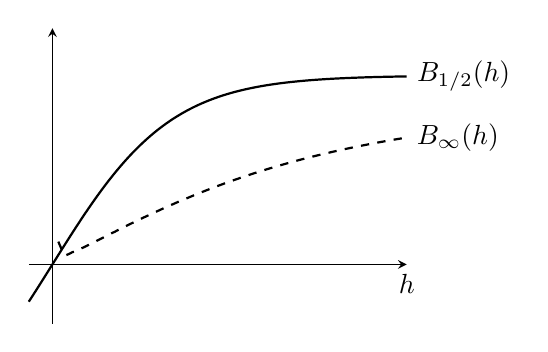
\begin{tikzpicture}[scale=1.5] 
      % \clip (-0.2,-0.5) rectangle (4.0,2.0);
      \draw[->,>=stealth,thin](-0.2,0)--(3,0)node[below]{$h$};
      \draw[->,>=stealth,thin](0,-0.5)--(0,2.0);
      \draw[samples=100,domain=-0.2:3.0,thick]plot(\x,{1.6*(tanh(\x))})node[right]{$B_{1/2}(h)$};
      \draw[samples=100,domain=0.05:3.0,thick,dashed]plot(\x,{1.6*(1/tanh(\x)-1/\x)})node[right]{$B_{\infty}(h)$};
    \end{tikzpicture} 
    \caption{$B_{1/2}(h)$と$B_{\infty}(h)$の図}
    \label{ans7}
  \end{figure}










\end{enumerate}












\end{document}
